\documentclass[11pt,a4paper]{article}

\usepackage[margin=2.2cm]{geometry}
\usepackage[T1]{fontenc}
\usepackage{lmodern}
\usepackage{amssymb}
\usepackage{xcolor}
\usepackage{tikz}
\usetikzlibrary{arrows.meta,positioning,fit,backgrounds,calc}
\usepackage{booktabs}
\usepackage{tabularx}
\usepackage{enumitem}
\usepackage{listings}
\usepackage[most]{tcolorbox}
\usepackage{fancyhdr}
\usepackage[colorlinks=true,linkcolor=blue!50!black,urlcolor=blue!50!black]{hyperref}

% ---------- colours ----------
\definecolor{local}{HTML}{2E7D32}
\definecolor{cloud}{HTML}{1565C0}
\definecolor{webc}{HTML}{EF6C00}
\definecolor{warn}{HTML}{C62828}
\definecolor{idea}{HTML}{6A1B9A}
\definecolor{soft}{HTML}{F5F5F5}

% ---------- boxes ----------
\newtcolorbox{concept}[1]{colback=idea!4,colframe=idea!70,fonttitle=\bfseries,title={Concept: #1},breakable}
\newtcolorbox{analogy}{colback=local!5,colframe=local!70,fonttitle=\bfseries,title={Analogy},breakable}
\newtcolorbox{why}{colback=cloud!4,colframe=cloud!70,fonttitle=\bfseries,title={Why it is done this way},breakable}
\newtcolorbox{caution}{colback=warn!4,colframe=warn!70,fonttitle=\bfseries,title={Watch out},breakable}
\newtcolorbox{exercise}{colback=soft,colframe=black!50,fonttitle=\bfseries,title={Check yourself},breakable}

\lstset{basicstyle=\ttfamily\small,backgroundcolor=\color{soft},frame=single,
        rulecolor=\color{black!25},columns=fullflexible,keepspaces=true,
        showstringspaces=false,breaklines=true}

\pagestyle{fancy}
\fancyhf{}
\lhead{\small Listen -- Learning Doc 02}
\rhead{\small Project Structure}
\cfoot{\thepage}

\title{\textbf{Listen}\\[4pt]\large Learning Doc 02: Project Structure\\
       \normalsize How code is organised into folders, and why}
\author{Detailed design, Section 1}
\date{6 October 2026}

\begin{document}
\maketitle

\begin{abstract}
\noindent Doc 01 decided the \emph{big pieces} of Listen (a laptop agent, a cloud API, a web
app). This document zooms in one level: how those pieces become \emph{folders and files} on
disk. It explains every folder and special file in the proposed layout (\texttt{app/},
\texttt{tests/}, \texttt{pyproject.toml}, and others you will meet soon), how the folders are
allowed to depend on each other, and, most importantly, a step-by-step method you could use
to arrive at this structure \emph{yourself}, without help.
\end{abstract}

\tableofcontents
\newpage

% =====================================================================
\section{Why folder structure matters at all}

A computer does not care where your code lives. You could put the entire project in one
10\,000-line file and Python would run it. Structure exists for \emph{humans}:

\begin{itemize}[nosep]
  \item \textbf{Finding things.} ``Where is the code that opens Google?'' should have an
        obvious answer.
  \item \textbf{Changing things safely.} If the speech code is in its own folder, editing it
        cannot accidentally break the sync code.
  \item \textbf{Understanding at a glance.} A good layout is a map of the system. Someone
        new should be able to read the folder names and roughly understand the project.
\end{itemize}

\begin{analogy}
A library could pile every book on the floor. All the books are still ``there'', but you
would never find one. Sections (science, history), shelves and call numbers do not change the
books; they make the library \emph{usable}. Folders are the sections of your codebase.
\end{analogy}

% =====================================================================
\section{The proposed layout}

\begin{lstlisting}
Listen/                          <- the repository (the whole project)
|-- agent/                       <- PROGRAM 1: runs on your laptop (Python)
|   |-- listen_agent/            <- the agent's actual code (a Python package)
|   |   |-- core/                   event bus, event types, config loading
|   |   |-- voice/                  listening modes, VAD, speech engines
|   |   |-- intent/                 recipe loading + matching
|   |   |-- actions/                open_url, launch_app, ... + executor
|   |   |-- usage/                  foreground-window tracker, title cleaner
|   |   |-- storage/                SQLite access
|   |   |-- sync/                   talks to the cloud API
|   |   `-- shell/                  terminal UI now, tray app later
|   |-- tests/                   <- automated checks for the agent
|   `-- pyproject.toml           <- the agent's "ID card + shopping list"
|-- server/                      <- PROGRAM 2: runs in the cloud (Python, FastAPI)
|   |-- app/                     <- the server's actual code (a Python package)
|   |   |-- routes/                 URL handlers (the API's front desk)
|   |   |-- services/               the real work (e.g. command_builder.py)
|   |   `-- models/                 shapes of data and database tables
|   |-- tests/
|   `-- pyproject.toml
|-- web/                         <- PROGRAM 3: runs in your browser (React)
|   |-- src/
|   `-- package.json             <- JavaScript's version of pyproject.toml
|-- shared/
|   `-- recipe.schema.json       <- the ONE definition of a valid command
`-- docs/
    |-- learning/                <- these PDFs
    `-- specs/                   <- design documents
\end{lstlisting}

\noindent The rest of this document walks through it from the outside in.

% =====================================================================
\section{Level 1: the repository}

\begin{concept}{Repository (repo)}
A \textbf{repository} is a project folder that \textbf{git} tracks. Git records every change
you \emph{commit}: what changed, when, and your message explaining why. You can go back to
any earlier version, compare versions, and later push the whole history to GitHub so a
deployment service can pull your code from there.
\end{concept}

\subsection{Monorepo vs.\ polyrepo}
We have three programs. They can live in one repository (\textbf{monorepo}) or three
(\textbf{polyrepo}).

\begin{center}
\renewcommand{\arraystretch}{1.25}
\begin{tabularx}{\textwidth}{l X X}
\toprule
 & \textbf{Monorepo (chosen)} & \textbf{Polyrepo} \\
\midrule
One change touching agent + server + web & One commit, reviewed together & Three commits in three repos, kept in step by hand \\
Sharing \texttt{recipe.schema.json} & Just a file in \texttt{shared/} & Copy it (copies drift) or publish it as a package \\
Who it suits & Solo devs, small teams, tightly linked programs & Big orgs with separate teams per program \\
\bottomrule
\end{tabularx}
\end{center}

\begin{why}
Adding one field to a command (say, a ``description'') touches all three programs. In a
monorepo that is one commit that tells the whole story. With three repos you would need to
remember to update all three, in the right order, every time.
\end{why}

\subsection{Pending decision: should \texttt{Listen/} be its own repo?}
Right now \texttt{Listen/} sits \emph{inside} a git repo called \texttt{LocalProject}, which
also contains an unrelated Node \texttt{package.json} and \texttt{index.js}. Options:
\begin{itemize}[nosep]
  \item \textbf{Make \texttt{Listen/} its own repo (recommended).} Its history contains only
        Listen. When you connect a deployment service or GitHub, you connect exactly this
        project. Nothing in \texttt{LocalProject} is deleted.
  \item \textbf{Keep it inside \texttt{LocalProject}.} Works, but every Listen commit sits
        alongside unrelated files, and deployment tools see a repo whose root is not your
        project.
\end{itemize}

% =====================================================================
\section{Level 2: one top-level folder per program}

\begin{concept}{Deployment unit}
A \textbf{deployment unit} is a piece of software that is installed and run \emph{as one
thing, in one place}. Listen has three:
\textcolor{local}{\texttt{agent/}} runs on your laptop,
\textcolor{cloud}{\texttt{server/}} runs on a cloud machine,
\textcolor{webc}{\texttt{web/}} is downloaded into a browser.
\end{concept}

The very first cut of the layout is: \textbf{one top-level folder per deployment unit}.
These three programs never share a running process; they only talk over the network. Giving
each its own folder makes that boundary physical: the cloud server is deployed from
\texttt{server/} alone and never even sees microphone code.

Two more top-level folders are \emph{not} programs:
\begin{itemize}[nosep]
  \item \texttt{shared/} holds \emph{agreements} between programs (Section~\ref{sec:shared}).
  \item \texttt{docs/} holds documents for humans.
\end{itemize}

% =====================================================================
\section{Level 3: inside a Python program}

\subsection{Files, modules and packages}
\begin{concept}{Module and package (Python)}
A \textbf{module} is one \texttt{.py} file. If you have \texttt{matcher.py}, other code can
write \texttt{import matcher}.

A \textbf{package} is a \emph{folder} of modules that Python can import as a group, written
with dots: \texttt{from listen\_agent.intent.matcher import match}. That one line says: in
package \texttt{listen\_agent}, sub-package \texttt{intent}, module \texttt{matcher}, take
\texttt{match}. The dots mirror the folders exactly.
\end{concept}

You already do this in your data-analysis work: when one script imports a prepared
DataFrame from another script, you are importing a module. A package is the same idea,
scaled up with folders.

\subsection{The project folder vs.\ the package folder}
Why \texttt{agent/listen\_agent/} and not just \texttt{agent/}? Because two different
things need a home:

\begin{center}
\renewcommand{\arraystretch}{1.2}
\begin{tabularx}{\textwidth}{l X}
\toprule
\texttt{agent/} (\textbf{project folder}) & Everything \emph{about} the program: its code, its tests, its
settings file, its README. Not importable. \\
\texttt{agent/listen\_agent/} (\textbf{package folder}) & \emph{Only} the code that actually runs. This is what
\texttt{import listen\_agent} loads. \\
\bottomrule
\end{tabularx}
\end{center}

\begin{why}
Tests and configuration are not part of the running program. If they lived inside the
package, they would be shipped and imported along with it. Keeping them next to the package,
not inside it, keeps the running program clean. The package gets a distinctive name
(\texttt{listen\_agent}, not \texttt{agent}) so it can never clash with some other
library also called \texttt{agent}.
\end{why}

\subsection{What \texttt{app/} means}
\texttt{server/app/} is the same idea as \texttt{agent/listen\_agent/}: the server's package
folder. Calling it \texttt{app} is simply the \textbf{convention} in the FastAPI world; the
official tutorials and templates use it, so anyone who has used FastAPI looks for
\texttt{app/} first.

\begin{concept}{Convention}
A \textbf{convention} is a choice that is not technically required but that a community has
agreed on, so everyone can read everyone else's projects. Following conventions is a gift to
your future self and to anyone who reads your code. Inventing your own names where a
convention exists is a cost, not a feature.
\end{concept}

\subsection{Inside \texttt{app/}: layers}
\begin{concept}{Layered architecture}
Split the server's code by \emph{kind of job}, and let each layer only call the layer below:
\begin{itemize}[nosep]
  \item \textbf{routes/}: the \emph{front desk}. Receives an HTTP request
        (``\texttt{GET /analytics/apps}''), checks it is well-formed, calls a service, sends
        back the answer. No real logic here.
  \item \textbf{services/}: the \emph{kitchen}. The actual work: computing top apps for a
        week, asking the LLM to draft a recipe, validating it.
  \item \textbf{models/}: the \emph{pantry labels}. Definitions of data shapes and database
        tables.
\end{itemize}
\end{concept}

\begin{analogy}
In a restaurant, the waiter takes your order and brings food but does not cook; the chef cooks
but never talks to customers. If you change the menu layout, the chef is unaffected. If you
change a recipe, the waiter is unaffected. Each layer can change without the other noticing.
\end{analogy}

\begin{center}
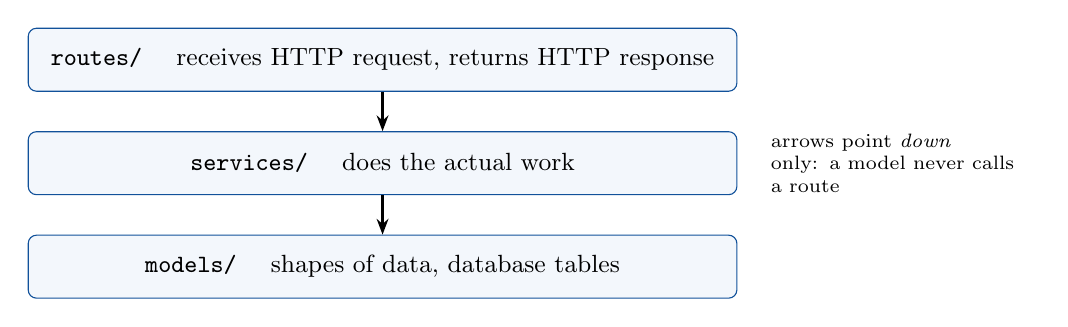
\begin{tikzpicture}[font=\small,
  lay/.style={draw=cloud!80!black,rounded corners=3pt,minimum width=9cm,minimum height=0.8cm,align=center,fill=cloud!5},
  arr/.style={-{Stealth[length=2mm]},thick}]
\node[lay] (r) {\texttt{routes/} \quad receives HTTP request, returns HTTP response};
\node[lay,below=0.5cm of r] (s) {\texttt{services/} \quad does the actual work};
\node[lay,below=0.5cm of s] (m) {\texttt{models/} \quad shapes of data, database tables};
\draw[arr] (r)--(s); \draw[arr] (s)--(m);
\node[right=0.3cm of s,align=left,font=\scriptsize,text width=3.3cm] {arrows point \emph{down}\\ only: a model never calls a route};
\end{tikzpicture}
\end{center}

\subsection{Inside \texttt{listen\_agent/}: one folder per box}
The agent's sub-folders are \emph{exactly} the boxes of the architecture diagram in Doc~01.
That is deliberate: the diagram becomes a map of the code.

\begin{center}
\renewcommand{\arraystretch}{1.2}
\begin{tabularx}{\textwidth}{l X X}
\toprule
\textbf{Folder} & \textbf{Its one job} & \textbf{Example files (later)} \\
\midrule
\texttt{core/}    & The shared plumbing: event bus, event definitions, settings & \texttt{bus.py}, \texttt{events.py}, \texttt{config.py} \\
\texttt{voice/}   & Microphone $\to$ text, in any of the 3 modes & \texttt{triggers/}, \texttt{vad.py}, \texttt{stt/} \\
\texttt{intent/}  & Text $\to$ ``which recipe, with which values'' & \texttt{recipes.py}, \texttt{matcher.py} \\
\texttt{actions/} & Actually do it: open a URL, change volume & \texttt{primitives.py}, \texttt{executor.py} \\
\texttt{usage/}   & Watch the foreground window, clean titles & \texttt{tracker.py}, \texttt{title\_cleaner.py} \\
\texttt{storage/} & Read/write the local SQLite file & \texttt{db.py} \\
\texttt{sync/}    & Exchange data with the cloud API & \texttt{client.py} \\
\texttt{shell/}   & What you see: terminal now, tray icon later & \texttt{terminal.py} \\
\bottomrule
\end{tabularx}
\end{center}

\noindent These file names are a preview. Every file will be introduced, with its reason, at
the moment we create it.

% =====================================================================
\section{\texttt{tests/}: code that checks code}

\begin{concept}{Automated test}
A \textbf{test} is a small function that runs a piece of your code with a known input and
checks the output is what you expect. A \textbf{test runner} (we use \textbf{pytest}) finds
all of them and runs them in seconds, printing which passed and which failed.
\end{concept}

\noindent A real example of what we will write:

\begin{lstlisting}[language=Python]
# agent/tests/intent/test_matcher.py
from listen_agent.intent.matcher import match

def test_search_extracts_query():
    result = match("search what is an atom")
    assert result.pattern == "search {query}"
    assert result.values["query"] == "what is an atom"
\end{lstlisting}

\noindent \texttt{assert} means ``this must be true, or the test fails''.

\begin{why}
Without tests, every change means manually saying ``Hey Jarvis, search\ldots'' to check you
did not break anything, across every command, every time. With tests, you run
\texttt{pytest} and in two seconds know that all 40 behaviours still work. Tests are what let
you change code \emph{without fear}. We will also write tests \emph{before} the code they
test (``test-driven development'', its own learning doc later).
\end{why}

\paragraph{Why \texttt{tests/} sits next to the package, and mirrors it.}
\texttt{tests/intent/test\_matcher.py} tests \texttt{listen\_agent/intent/matcher.py}.
Mirroring means that for any code file you instantly know where its tests are. Pytest finds
tests automatically by name: any file called \texttt{test\_*.py}, any function called
\texttt{test\_*}. That naming is another convention.

% =====================================================================
\section{\texttt{pyproject.toml}: the program's ID card and shopping list}

\subsection{What TOML is}
\textbf{TOML} is just a text format for settings, designed to be easy for humans to read:
\texttt{key = value}, grouped under \texttt{[section]} headings. Nothing more magical than
that.

\subsection{What \texttt{pyproject.toml} says}
It is the \textbf{one file that describes a Python project} to tools. A shortened version of
what the agent's will look like:

\begin{lstlisting}
[project]
name = "listen-agent"                 # the program's name
version = "0.1.0"                     # its version
requires-python = ">=3.11"            # which Python it needs
dependencies = [                      # libraries it needs to RUN
    "faster-whisper",
    "openwakeword",
    "sounddevice",
]

[dependency-groups]
dev = ["pytest", "ruff"]              # libraries only needed while DEVELOPING

[tool.pytest.ini_options]             # settings for the test runner
testpaths = ["tests"]
\end{lstlisting}

\begin{concept}{Dependency}
A \textbf{dependency} is someone else's code that your program needs, such as
\texttt{faster-whisper} for speech recognition. You do not copy it into your project; you
\emph{declare} it, and a tool downloads the right version.
\end{concept}

\begin{analogy}
\texttt{pyproject.toml} is a recipe card's ingredient list. It does not contain the flour;
it says ``200\,g flour''. Anyone (or any deployment server) can read the list and fetch
exactly the same ingredients.
\end{analogy}

You have actually seen this idea already: the \texttt{package.json} in your
\texttt{LocalProject} folder is the JavaScript world's version of exactly the same file.

\subsection{Why each Python program has its \emph{own} \texttt{pyproject.toml}}

\begin{concept}{Virtual environment}
A \textbf{virtual environment} (venv) is a private, isolated set of installed libraries for
one project. Installing something in one venv does not affect any other venv or your system
Python. Each \texttt{pyproject.toml} gets its own venv.
\end{concept}

The agent and the server need \emph{different} ingredients:
\begin{itemize}[nosep]
  \item The \textbf{agent} needs microphone, speech and Windows libraries.
  \item The \textbf{server} needs FastAPI and a PostgreSQL driver.
\end{itemize}
If they shared one list, the cloud server would have to install microphone and speech
libraries it can never use (wasting space, slowing deploys, and possibly failing to install
on a Linux server with no audio hardware), and your lightweight agent would carry a web
framework. Separate files mean each program installs only what it uses.

\subsection{The files that appear next to it}
\begin{center}
\renewcommand{\arraystretch}{1.2}
\begin{tabularx}{\textwidth}{l X}
\toprule
\texttt{uv.lock} & Created automatically. Records the \emph{exact} version of every library
(and the libraries \emph{they} depend on). \texttt{pyproject.toml} says ``faster-whisper,
roughly this version''; the lock file says ``exactly 1.1.0, and exactly these 27 sub-libraries''.
So your laptop and the server get identical installs. Never edited by hand. \\
\texttt{.venv/} & The virtual environment itself: the downloaded libraries. Large, rebuilt
any time from the lock file, so it is \emph{not} saved in git. \\
\texttt{README.md} & A short human guide: what this program is, how to install and run it. \\
\bottomrule
\end{tabularx}
\end{center}

\paragraph{The tools.} \textbf{uv} reads \texttt{pyproject.toml}, creates the venv, installs
dependencies and writes the lock file (it replaces \texttt{pip} + \texttt{venv}).
\textbf{ruff} reads your code and flags likely mistakes (unused imports, undefined names)
before you even run it.

% =====================================================================
\section{\texttt{web/}: the JavaScript side}
React projects have their own conventions, created for us by a setup tool:
\begin{itemize}[nosep]
  \item \texttt{package.json}: the same role as \texttt{pyproject.toml}: name, dependencies,
        and commands like \texttt{npm run dev}.
  \item \texttt{src/}: the source code (pages, components). Equivalent of the package folder.
  \item \texttt{node\_modules/}: downloaded libraries, the equivalent of \texttt{.venv/};
        never committed to git.
\end{itemize}
We will cover these in detail in the web-app learning doc.

% =====================================================================
\section{\texttt{shared/}: one agreement, read by everyone}\label{sec:shared}

\begin{concept}{Contract and single source of truth}
When several programs must agree on something, write that agreement down \textbf{once}, in
one place, and have every program read it. That file is the \textbf{contract}.
\end{concept}

A command recipe is created in the web app, stored by the server, and executed by the agent.
All three must agree on what a valid recipe is (it must have a \texttt{pattern}; the
\texttt{action} must be one of the known primitives; \ldots). \texttt{recipe.schema.json} is
a \textbf{JSON Schema}: a file that describes the allowed shape of some data, which libraries
in both Python and JavaScript can check data against.

\begin{caution}
The alternative, writing the rules separately in Python (twice) and in JavaScript, works on
day one. Months later someone updates one copy and forgets the others; the web app happily
saves a recipe that the agent rejects. Duplicated rules \emph{always} drift apart eventually.
\end{caution}

% =====================================================================
\section{How the folders interact}

This is the most important section. A structure is defined not just by its folders but by
\textbf{who is allowed to depend on whom}.

\begin{concept}{Dependency direction}
``A depends on B'' means A's code uses B (imports it, or calls it over the network). If B
changes, A may break. Good structures make dependencies point in \emph{one direction} and
never form a circle (A needs B needs C needs A), because a circle means nothing can be
changed or tested on its own.
\end{concept}

\subsection{Between programs: only over the network}
\begin{center}
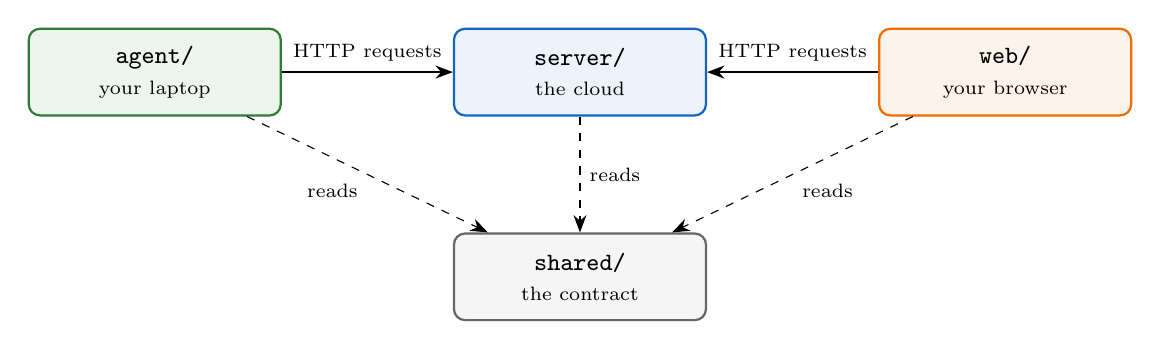
\begin{tikzpicture}[font=\small,
  prog/.style={draw,rounded corners=4pt,minimum width=3.2cm,minimum height=1.1cm,align=center,thick},
  arr/.style={-{Stealth[length=2.2mm]},thick},
  rd/.style={-{Stealth[length=2.2mm]},dashed}]
\node[prog,draw=local,fill=local!8] (a) at (0,0) {\texttt{agent/}\\\scriptsize your laptop};
\node[prog,draw=cloud,fill=cloud!8] (s) at (5.4,0) {\texttt{server/}\\\scriptsize the cloud};
\node[prog,draw=webc,fill=webc!8] (w) at (10.8,0) {\texttt{web/}\\\scriptsize your browser};
\node[prog,draw=black!60,fill=soft] (sh) at (5.4,-2.6) {\texttt{shared/}\\\scriptsize the contract};
\draw[arr] (a) -- node[above,font=\scriptsize]{HTTP requests} (s);
\draw[arr] (w) -- node[above,font=\scriptsize]{HTTP requests} (s);
\draw[rd] (a) -- node[below left,font=\scriptsize]{reads} (sh);
\draw[rd] (s) -- node[right,font=\scriptsize]{reads} (sh);
\draw[rd] (w) -- node[below right,font=\scriptsize]{reads} (sh);
\end{tikzpicture}
\end{center}

\noindent The rules:
\begin{enumerate}[nosep]
  \item \texttt{agent/} \textbf{never imports} from \texttt{server/}, and vice versa. They are
        different machines; the only way they talk is HTTP requests to the API.
  \item \texttt{web/} talks \emph{only} to the server's API, never to a database.
  \item The server never calls the agent or the web app. They call it. (The agent
        \emph{asks} the server ``any command changes for me?''; the server never reaches out
        to your laptop. This is why sync works even when your laptop is behind home Wi-Fi.)
  \item Everyone may \emph{read} \texttt{shared/}; \texttt{shared/} depends on nothing.
\end{enumerate}

\subsection{Inside the agent: everything goes through \texttt{core/}}
\begin{center}
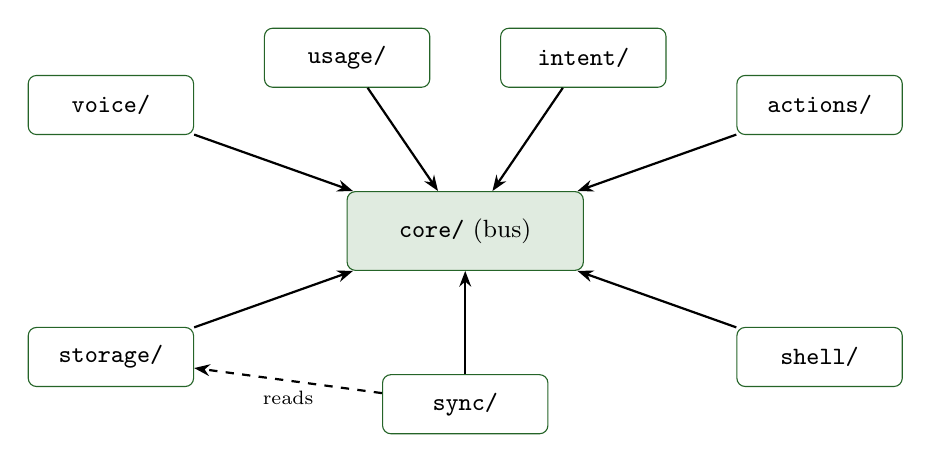
\begin{tikzpicture}[font=\small,
  m/.style={draw=local!80!black,rounded corners=3pt,minimum width=2.1cm,minimum height=0.75cm,fill=white},
  arr/.style={-{Stealth[length=2mm]},thick}]
\node[m,fill=local!15,minimum width=3cm,minimum height=1cm] (core) at (0,0) {\textbf{\texttt{core/}} (bus)};
\node[m] (voice)  at (-4.5, 1.6) {\texttt{voice/}};
\node[m] (usage)  at (-1.5, 2.2) {\texttt{usage/}};
\node[m] (intent) at ( 1.5, 2.2) {\texttt{intent/}};
\node[m] (act)    at ( 4.5, 1.6) {\texttt{actions/}};
\node[m] (stor)   at (-4.5,-1.6) {\texttt{storage/}};
\node[m] (sync)   at ( 0,  -2.2) {\texttt{sync/}};
\node[m] (shell)  at ( 4.5,-1.6) {\texttt{shell/}};
\foreach \n in {voice,usage,intent,act,stor,sync,shell} \draw[arr] (\n) -- (core);
\draw[arr,dashed] (sync) -- node[below,font=\scriptsize]{reads} (stor);
\end{tikzpicture}
\end{center}

\noindent Every module depends on \texttt{core/} (to publish and subscribe to events), and
\texttt{core/} depends on none of them. Modules do not import each other, with one
justified exception: \texttt{sync/} reads from \texttt{storage/} to find what to upload.

\begin{why}
Because \texttt{voice/} does not import \texttt{intent/}, you can test the matcher without a
microphone, and replace the speech engine without touching the matcher. Because
\texttt{core/} depends on nothing, it is stable: the piece everything relies on is the piece
that changes least. That is the property you want.
\end{why}

\subsection{One command, traced through the files}
``Hey Jarvis\ldots search what is an atom'':
\begingroup\sloppy
\begin{enumerate}[nosep]
  \item \texttt{shell/terminal.py} starts the program and starts each module's thread.
  \item \texttt{voice/} hears the wake word, transcribes, publishes \texttt{CommandHeard} via \texttt{core/bus.py}.
  \item \texttt{intent/matcher.py} (subscribed) matches the recipe \texttt{search \{query\}}, publishes \texttt{IntentMatched}.
  \item \texttt{actions/executor.py} (subscribed) runs the primitive \texttt{open\_url}, then
        publishes \texttt{CommandExecuted}.
  \item \texttt{storage/db.py} (subscribed) writes the event to SQLite; \texttt{shell/} prints it.
  \item Minutes later, \texttt{sync/client.py} reads unsent rows and sends them to
        \texttt{server/app/routes/}, which calls \texttt{services/}, which saves them using
        \texttt{models/}.
  \item \texttt{web/src/} asks the server for analytics, and the command shows up on your dashboard.
\end{enumerate}
\endgroup

% =====================================================================
\section{Code vs.\ data: what goes in the repo}

\begin{concept}{Code vs.\ user data vs.\ secrets}
\begin{itemize}[nosep]
  \item \textbf{Code} (and default settings) goes in the repo, so it is versioned and shared.
  \item \textbf{Your data} (the SQLite database, your edited command list, logs) lives
        \emph{outside} the repo, in your Windows user-data folder
        (\texttt{\%APPDATA\%\textbackslash Listen}). It is personal, it changes every
        second, and it must never end up on GitHub.
  \item \textbf{Secrets} (the LLM API key, database passwords) live in a \texttt{.env} file that
        git is told to ignore. The repo contains a \texttt{.env.example} with empty
        values, so you remember which secrets are needed.
\end{itemize}
\end{concept}

\noindent \textbf{\texttt{.gitignore}} is the file that tells git which things to never track:
\texttt{.venv/}, \texttt{node\_modules/}, \texttt{.env}, database files. Putting a secret in
git is one of the most common (and serious) beginner mistakes: once it is pushed, assume it is
public, even if you delete it later.

% =====================================================================
\section{How would you come up with this yourself?}

Nobody invents a layout from nothing. Here is a method you can reuse on any future project.
Each step is a question; the answers \emph{produce} the structure.

\begin{enumerate}
  \item \textbf{Where does each thing run?}\\
        List the places code runs: laptop, cloud, browser. \emph{Each place becomes a top-level
        folder.} (This gave us \texttt{agent/}, \texttt{server/}, \texttt{web/}.)

  \item \textbf{What does each program need to install?}\\
        If two programs need different libraries, they need separate dependency files and
        environments. (One \texttt{pyproject.toml} each.)

  \item \textbf{What are the jobs inside each program?}\\
        Write the requirements as sentences, underline the verbs: \emph{listen},
        \emph{understand}, \emph{act}, \emph{track}, \emph{store}, \emph{sync},
        \emph{display}. Each distinct job is a candidate folder.

  \item \textbf{Would these two things change for different reasons?}\\
        This is the key test, often called the \textbf{single-responsibility principle}.
        Swapping the speech engine and adding a new command are unrelated changes, so speech
        code and matching code go in different folders. If two things always change together,
        keep them together.

  \item \textbf{Draw the arrows: who needs whom?}\\
        Sketch boxes and dependency arrows. If you find a circle, introduce something in the
        middle that both sides depend on instead (that is exactly what \texttt{core/}'s event
        bus is for).

  \item \textbf{What is shared between programs?}\\
        Anything two programs must agree on becomes a single contract file (\texttt{shared/}).

  \item \textbf{What does the community already do?}\\
        Before inventing names, look at the official tutorial or project template for each
        tool (FastAPI's docs use \texttt{app/}; pytest expects \texttt{tests/} and
        \texttt{test\_*.py}; React's setup tool creates \texttt{src/}). Reading the folder
        layout of a few well-known open-source projects on GitHub is one of the best ways to
        learn this.

  \item \textbf{Start small; let it grow.}\\
        You do not need every folder on day one. Create a folder when its first file appears.
        When a file grows past a few hundred lines or starts doing two jobs, split it.
        Structure is refactored as you learn, not fixed forever.
\end{enumerate}

\begin{caution}
Honest note: the first time, your structure will be imperfect, and that is fine. Experienced
developers mostly have better \emph{instincts} for step 4 (``would these change for different
reasons?''), built from past mistakes. Using the questions above deliberately is how you build
that instinct faster.
\end{caution}

% =====================================================================
\section{Glossary}
\begin{description}[style=nextline,leftmargin=1.2cm,itemsep=2pt]
  \item[\texttt{.env} / \texttt{.env.example}] File of secrets (ignored by git) / its empty template (committed).
  \item[\texttt{.gitignore}] List of files and folders git must never track.
  \item[\texttt{app/}] Conventional name for a FastAPI server's package folder.
  \item[Contract] A single written agreement that several programs follow.
  \item[Convention] A community-agreed naming or layout choice.
  \item[Dependency] Someone else's code your program needs; declared, not copied.
  \item[Deployment unit] Software installed and run as one thing in one place.
  \item[JSON Schema] A file describing the allowed shape of JSON data.
  \item[Layered architecture] Code split into layers (routes, services, models), each calling only the layer below.
  \item[Lock file] Exact versions of every installed library (\texttt{uv.lock}).
  \item[Module / package] One \texttt{.py} file / a folder of modules.
  \item[Monorepo] One repository holding several related programs.
  \item[\texttt{pyproject.toml}] The file describing a Python project: name, Python version, dependencies, tool settings.
  \item[Repository] A folder whose history git tracks.
  \item[Single-responsibility principle] Group code by its reason to change.
  \item[Test / test runner] Code that checks code / the tool (pytest) that runs the checks.
  \item[TOML] A simple \texttt{key = value} settings format.
  \item[Virtual environment] An isolated set of installed libraries for one project.
\end{description}

% =====================================================================
\section{Check your understanding}
\begin{exercise}
\begin{enumerate}
  \item Why is there a \texttt{pyproject.toml} in \texttt{agent/} \emph{and} in
        \texttt{server/}, instead of one at the top?
  \item What is the difference between \texttt{agent/} and \texttt{agent/listen\_agent/}?
  \item A new route \texttt{GET /analytics/top-apps} needs to compute the top 5 apps. Which
        file in \texttt{server/app/} receives the request, and which does the computing?
  \item Why may \texttt{intent/} not import \texttt{voice/}? What would you lose?
  \item Where does your SQLite database file live, and why not inside the repo?
  \item You need to add a tray icon. Using the method in Section 12, which folder does it go
        in, and why does nothing else need to change?
  \item Suppose \texttt{web/} kept its own copy of the recipe rules instead of reading
        \texttt{shared/}. Describe a realistic bug that would appear months later.
\end{enumerate}
\end{exercise}

\end{document}
